\documentclass[10pt,a4paper]{article}
\usepackage[utf8]{inputenc}
\usepackage[T1]{fontenc}
\usepackage{amsmath}
\usepackage{amssymb}
\usepackage{graphicx}

\usepackage{hyperref}
%\usepackage{url}
\usepackage{xspace}
\usepackage{float}
\restylefloat{figure}



\usepackage{tikz}
\usepackage{xcolor}
\definecolor{corn}{rgb}{0.98, 0.93, 0.36}
\definecolor{emerald}{rgb}{0.31, 0.78, 0.47}

\usetikzlibrary{positioning,patterns,arrows,decorations.markings,decorations.pathreplacing,shapes,shapes.misc}


\def\non{\nonumber}
\def\p{\partial}
\def\o{\over}



\title{Summary of pyVRS Non-Dimensionalization for the Semi-Spheroid Chimera Model of Embryo Swimming}
\author{Daniel Gr\"unbaum}

\begin{document}
\maketitle
This document summarizes one approach to nondimensionalizing the equatioins, code and parameter space underlying the semi-spheroid chimera model of embryo swimming, as implemented in pyVRS. 
The fundamental shapes in this model are chimeras constructed from two attached semi-spheroids, matched in radius but usually differing in height. 
We refer to a chimera of this type as a ``constitutive chimera''.

One instance of a constitutive chimera represents the surface of the embryo.
The volume inside this surface is assumed to be (mostly) tissue. 
Other constitutive chimeras may be used to approximate inclusions, containing material such as seawater or lipid (both less dense than tissue) or calcium carbonate (heavier than tissue).
If the volume of tissue is held constant, inclusions alter the volume enclosed by the surface, and typically shift the center of gravity away from the center of buoyancy.
A shift of this type results in a preferred orientation, in still water.

The ability of the embryo to swim directionally (typically upwards) depends on the relative strengths of the ``body-force'' righting moments, associated with gravity and buoyancy, compared to destabilizing environmental moments from shear and vorticity that tend to turn larvae away from their vertical orientations.
The overarching goals of the analysis are to:
\begin{enumerate}
	\item Assess how embryo size and morphology affects body-force righting moments and destabilizing environmental moments; 
	\item Assess habitats and conditions under which environmental moments exceed righting moments, compromising embryos' capacities for oriented swimming; and 
	\item Assess whether existing or hypothetical embryo sizes and morphologies are likely to encounter habitat-specific constraints, and whether observed patterns of size and morphology are consistent with predictions stemming from a requirement for oriented swimming.
\end{enumerate}
In this analysis we consider only chimeras comprising semi-spheroids.
We do not consider the more general case of semi-ellipsoids with radially asymmetrical shapes.
We also restrict our analysis to embryo shapes that are overall radially symmetrical -- that is, embryos constructed from semi-spheroids aligned along the vertical axis. 
This is in part to avoid a proliferation of parameter space, but mostly because the observed larval shapes approximate our focal class of morphologies. 
We note, though, that it is an interesting open question why early stage embryos are typically radially symmetrical\footnote{One hypothesis is that most or all such asymmetries would decrease initial stability.}. 

\section{Basic geometry of a semi-spheroid chimera}

\begin{figure}[t] 
	\begin{center}
		\resizebox{6.5cm}{!}{
			
			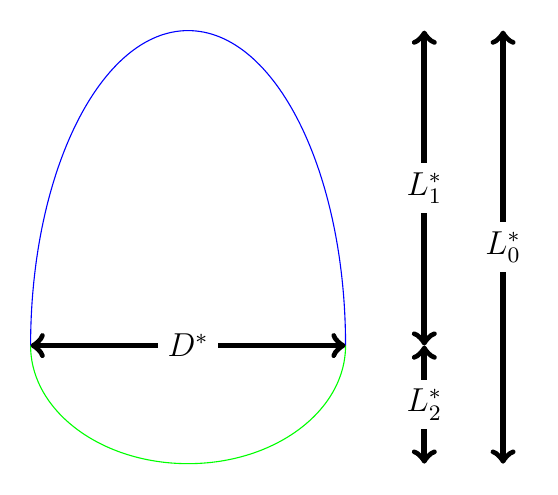
\begin{tikzpicture}
				%\draw (0,0) ellipse (2cm and 1cm);
				%\draw (0,3) ellipse (2cm and 1cm);
				%\draw (-3,1.5) +(60:1cm and 2cm) arc (60:-240:1cm and 2cm);
				%\draw (0,0) +(180:1cm and 2cm) arc (90:270:1cm and 2cm);
				% Arc operation
				\draw[blue] (2,0) arc
				[
				start angle=0,
				end angle=180,
				x radius=2cm,
				y radius =4cm
				] ;
				\draw[green] (2,0) arc
				[
				start angle=0,
				end angle=-180,
				x radius=2cm,
				y radius =1.5cm
				] ;
				\coordinate []  (A) at (-2,0)  ;
				\coordinate []  (B) at (2,0) ;
				\coordinate []  (A1) at (3,4)  ;
				\coordinate []  (B1) at (3,-1.5) ;		
				\coordinate []  (A2) at (4,4)  ;
				\coordinate []  (B2) at (4,-1.5) ;		
				\coordinate []  (equator) at (3,0) ;
				\coordinate []  (equator2) at (4,0) ;
				%		\coordinate [label=-90:$A$]  (A) at (-2,0)  ;
				%		\coordinate [label=90:$B$ ]  (B) at (2,0) ;
				%\node (A) [draw=black,fill=emerald,double=white,double distance=2pt,shape=rounded rectangle,minimum width=4cm ]{A}; 
				%\node[right=9cm of A] (B) [draw,fill=corn,shape=rounded rectangle,minimum width=4cm ]{B};
				\path[<->] (A) edge[line width=0.742mm] node[ fill=white, anchor=center, pos=0.5,font=\bfseries] {\large $D^*$} (B);
				\path[<->] (equator) edge[line width=0.742mm] node[ fill=white, anchor=center, pos=0.5,font=\bfseries] {\large $L_1^*$} (A1);
				\path[<->] (equator) edge[line width=0.742mm] node[ fill=white, anchor=center, pos=0.5,font=\bfseries] {\large $L_2^*$} (B1);
				\path[<->] (A2) edge[line width=0.742mm] node[ fill=white, anchor=center, pos=0.5,font=\bfseries] {\large $L_0^*$} (B2);
			\end{tikzpicture}
		}
	\end{center}
	\caption{Layout of a constitutive chimera, in profile view. The view represents a vertical cross-section of a shape that is radially symmetrical about the vertical axis. The upper semi-spheroid, with diameter $D$ and height $L_1$, is shown in blue. The lower semi-spheroid, with diameter $D$ and height $L_2$, is shown in green. } \label{chimera1}
\end{figure}
\noindent
Figure \ref{chimera1} presents a schematic of a constitutive chimera.
A constitutive chimera is parameterized by:
\begin{itemize}
	\item $D^*$, the shared diameter of its upper and lower semi-spheroids;
	\item $L_1^*$, the height of its upper semi-spheroid;
	\item $L_2^*$, the height of its  lower semi-spheroid; 
	\item $L_0^* \equiv L_1^* + L_2^*$, the total height of the chimera; and,
	\item $\alpha \equiv \frac{L_0^*}{D^*}$, an aspect ratio parameter.
\end{itemize}
We refer to the junction between the upper and lower semi-spheroids (indicated by $D$ in Figure \ref{chimera1}) as the ``equator''.
The asterisks imply dimensional quantities.

From the formula for the volume of an spheroid, applied to each semi-spheroid and summed, the total volume of a constitutive chimera is
\begin{equation}\label{vol1}
	V^* = \frac{\pi}{6} {D^*}^2 \left(\frac{L_1^*+L_2^*}{2}\right) = \frac{\pi}{12} {D^*}^2 L_0^*
\end{equation} 
Equation \ref{vol1} shows that the volume is a function of diameter and total length, $L_0^*$, regardless of how that length is allocated to the upper or lower semi-spheroids.
The volume can also be expressed in terms of the aspect ratio,
\begin{equation}\label{vol2}
	V^* = \frac{\pi}{12} \alpha {D^*}^3
\end{equation} 
From a morphological perspective, this implies that an embryo of fixed height $L_0^*$ can develop into a constitutive chimera with any aspect ratio, without a change in tissue volume. 

This convenient fact suggests a nondimensionalizations based on an equivalent spherical diameter, defined as the diameter of the sphere with volume equal to that of the surface (tissue) constitutive chimera:
\begin{equation}\label{equivsphere}
	V_{sph}^* = \frac{\pi}{6} {D_{sph}^*}^3
\end{equation} 
Equating the spherical volume to the right hand side of Equation \ref{vol2} simplifies to
\begin{equation}\label{equivD}
	D_{sph}^* = \sqrt[\uproot{5}3]{\frac{\alpha}{2}} ~ D^*
\end{equation} 

We adopt $D_{sph}^*$ as the characteristic length for nondimensionalizing embryo morphology.
For example, a nondimensionalized chimera diameter is
\begin{equation}\label{ndD}
	D = \frac{D^*}{D_{sph}^*}
\end{equation} 
where the dropped asterisk implies a nondimensional quantity.

Because $D_{sph}^*$ is defined to match volumes, this also ensures that the nondimensional volume of the tissue is equal to 1.
As a result, the body forces (excluding effects of inclusions) are also normalized to remove the primary effects of size.


\section{Rotational movement of a sphere}
The rotation rate of a sphere of diameter $D_{sph}^*$ in a fluid of viscosity $\mu$ is 
\begin{equation}\label{rot1}
	\omega^* = \frac{T^*}{\pi \mu {D^*}^3} = \frac{T^*}{6 \mu V_{sph}^*},	
\end{equation}
where $T^*$ is the imposed torque (i.e., the imposed moment).

We can define a rotation timescale, $\tau_{rot}^*$, as the inverse of this rate,
\begin{equation}\label{tau1}
	\tau_{rot}^* \equiv {\omega^*}^{-1} = \frac{\pi \mu {D^*}^3}{T^*} = \frac{6 \mu V_{sph}^*}{T^*}
\end{equation}

For the timescale $\tau_{rot}^*$ to reflect the fundamental effects of size on chimera swimming, we can choose a value of $T^*$ that emerges from the equivalent sphere.
Specifically, Equation \ref{equivsphere} gives a characteristic buoyancy force of
\begin{equation}\label{charF}
	F_{sph}^* = \frac{\pi}{6} \rho_{med}^* g {D_{sph}^*}^3 = \rho_{med}^* g V_{sph}^*,
\end{equation} 
where $\rho_{med}^*$ is the density of the fluid medium, and $g$ is gravitational acceleration.
Again using $D_{sph}^*$ as a characteristic length (in this case, the distance over which the characteristic force acts to generate a moment), we can assign a characteristic value to the torque:
\begin{equation}\label{charT}
	T^* = F_{sph}^* D_{sph}^* = \frac{\pi}{6} \rho_{med}^* g {D_{sph}^*}^4 = \rho_{med}^* g D_{sph}^* V_{sph}^*,
\end{equation} 
This torque is an upper limit that cannot be realized (or, in most reasonable geometries, even approached).
This is because the body forces generated by inclusions will rarely approach the body force of the tissue, and the moment arm over which inclusion forces act will rarely approach the entire length of the embryo. 
Nonetheless, this torque is likely to scale in a similar way with embryo size, and the viscosity and density of the fluid medium, as torques on more realistic embryo shapes. This makes it is suitable as a characteristic value to factor out direct effects of those parameters.

Substituting this value into Equation \ref{tau1} and simplifying gives
\begin{equation}\label{tau2}
	\tau_{rot}^* = 6 \frac{\mu}{\rho^* g D_{sph}^*}
\end{equation}
Equation \ref{tau2} reflects the fundamental proportional dependence of the rotation timescale of an equivalent sphere on size (diameter), viscosity, medium density, and gravitational acceleration.


\section{Non-dimensionalized Stokes Equations}

\begin{equation}\label{Stokes1}
	0 = \mu \left( \frac{\p^2 u^*}{\p {x^*}^2}+\frac{\p^2 v^*}{\p {y^*}^2}+\frac{\p^2 w^*}{\p {z^*}^2} \right) - \frac{\p p^*}{\p {x^*}} + f_x^*
\end{equation}

Take:
\begin{itemize}
	\item $x^* = D_{sph} x$, $x = \frac{x^*}{D_{sph}}$
	\item $u^* = \frac{D_{sph}}{\tau_{rot}} u$, $u = \frac{\tau_{rot}}{D_{sph}} u^*$
	\item $f_x^* = \frac{\mu}{\tau_{rot} D_{sph}} f_x$, $f_x = \frac{\tau_{rot} D_{sph}}{\mu} f_x^*$
	\item $p^* = \frac{\mu}{\tau_{rot}} p$, $p = \frac{\tau_{rot}}{\mu} p^*$
\end{itemize}


\begin{equation}\label{blah3}
	u = 6 \frac{\mu}{\rho^* g } u^*
\end{equation}
\begin{equation}\label{blah}
	f_x = \frac{D_{sph}}{\mu} 6 \frac{\mu}{\rho^* g D_{sph}^*} f_x^* = \frac{6}{\rho g} f_x^*
\end{equation}
\begin{equation}\label{blah2}
	p = \frac{1}{\mu} 6 \frac{\mu}{\rho^* g D_{sph}^*} p^* = \frac{6}{\rho g D_{sph}^*} p^*
\end{equation}

\begin{equation}\label{Stokes2}
	0 = \left( \frac{\p^2 u}{\p x^2}+\frac{\p^2 v}{\p y^2}+\frac{\p^2 w}{\p z^2} \right) - \frac{\p p}{\p x} + f_x
\end{equation}

%\vspace{10cm}
%\begin{tikzpicture}
%	\draw (0,0) ellipse (2cm and 1cm);
%	\draw (0,3) ellipse (2cm and 1cm);
%	\draw (-3,1.5) +(60:1cm and 2cm) arc (60:-240:1cm and 2cm);
%	\node (A) [draw=black,fill=emerald,double=white,double distance=2pt,shape=rounded rectangle,minimum width=4cm ]{A}; 
%	\node[right=9cm of A] (B) [draw,fill=corn,shape=rounded rectangle,minimum width=4cm ]{B};
%	\path[->] (A) edge[line width=0.742mm] node[ fill=white, anchor=center, pos=0.5,font=\bfseries] {\Huge +} (B);
%\end{tikzpicture}













\end{document}